\section{Desarrollo}

\subsection{Interpolación}

Interpolar consiste en estimar valores desconocidos en base a otros ya conocidos dados por un \textit{data-set} predefinido, que suponemos sugiere el comportamiento de alguna función \textit{f} para la cual solo conocemos una cantidad determinada de resultados. Estos datos suelen organizarse en tablas de pares $(x_i,y_i)$, donde $y_i$ es el $f(x_i)$ y $x_i$ es algún valor conocido del dominio de \textit{f} sobre el cual deseamos trabajar; dicho esto el problema entonces se traduce en aproximar dicha función, procurando satisfacer la obvia restricción de \textit{matchear} con esos valores ya conocidos bajo sus respectivas pre-imagenes. Para ello existen diversos metodos algoritmicos que en base a nuestros datos intentan generar esa función aproximada, entre ellos por ejemplo, se encuentran los metodos de interpolación polinomial que como su nombre sugiere intentan lograrlo por medio de algún polinomio (al que llamamos polinomio interpolador). 

%\subsection{Polinomio interpolador}

%Interpolar significa estimar el valor desconocido de una función en un punto,
%ponderando sus valores conocidos para puntos intermedios. Para lograrlo podemos construir un polinomio en base a estos valores conocidos. La presición dependerá del polinomio elegido y siempre se dispondrá de una formula para el error que permitirá ajustarla.
%Aplicativamente, esto tendrá sentido siempre y cuando no dispongamos de la función real o que computacionalmente no sea viable debido a la complejidad involucrada para data sets muy grandes. En general, los polinomios son menos costosos y muy flexibles computacionalmente.

\subsection{Interpolación polinómica}

Dada una función $f$ de la cual se conocen sus valores en un número finito de puntos $x_0$, $x_1$, ..., $x_m$, con $m \in \mathbb{N}$, se llama interpolación polinómica al proceso de hallar un polinomio $P_m(x)$ de grado menor o igual a $m$, cumpliendo $P_m(x_k)$ = $f(x_k)$,  $\forall$ $k$ = 0, 1, ..., $m$.
Este polinomio se conoce como polinomio interpolador y tendrá la siguiente forma:

\begin{equation}
	 P_m(x) = a_mx^m + a_{m-1}x^{m-1} + \dots + a_1x + a_0
\end{equation}

Donde $a_m$, $a_{m-1}$, $\dots$, $a_1$, $a_1$ $\in \mathbb{R}$.

Este tipo de interpolación suele considerarse para aproximar funciones continuas, esto es asi porque los polinomios tiene buenas propiedades analiticas, entre las cuales podemos considerar las siguientes: son continuas, facilmente integrables e infinitamente derivables (pertenecen a la clase $C^{\infty}[a, b]$), y además sus derivadas y primitivas son a su vez polinomios. Otro propiedad importante de la cual se fundamenta este tipo de interpolación es la de que dada cualquier funcion definida y continua en un intervalo cerrado y acotado, existe un polinomio que aproxima tanto como se desee a esa función; formalmente esto es enunciado mediante el siguiente teorema.

%Otra razon importante para considerar esta clase de polinomios es que sus derivadas e integrales indefinidas son fáciles de calcular y además tambien son polinomios. Por esta razon los polinomios interpoladores son utilizados para interpolar funciones continuas.
%Un motivo de su importancia es que aproximan uniformemente funciones continuas. 
%Con esto queremos decir que dada cualquier funcion definida y continua en un intervalo cerrado, existe un polinomio que aproxima tanto como sea deseado a esa función.

\begin{theorem}
	\item Weierstrass Aproximation Theorem
	\item Supongamos que $f$ es definida y continua en $[a, b]$. Para cada $\epsilon > 0$, existe un polinomio $P(x)$ con la siguiente propiedad:	
\end{theorem}
\begin{equation}
	 |f(x) - P(x)| < \epsilon, \forall x \in [a, b]
\end{equation}

La demostración de este teorema puede encontrarse en textos de análisis real o documentos universitarios.(crear una cita a http://www.math.harvard.edu/~waffle/wapproxt.pdf).\vspace{2mm}
\\
 Dado el anterior teorema podemos considerar a nuestra función \textit{f} como algún polinomio interpolador mas otra función de corrección a la que denominaremos la expresión del error. Esta última función correjirá la inprecisión del polinomio con respecto a la función original para cada valor de su dominio. No obstante puede que encontrar dicha expresion no sea para nada trivial.

 %Podremos entonces, además, obtener la expresion del error de aproximación del polinomio. La misma nos servirá para ajustar el paso que deberemos tomar cuando deseamos acotar el error. 

%\begin{theorem}
%	\item Sean $x_0$, $x_1$, ..., $x_m$ en el intervalo $[a, b]$ y $f \in C^{m+1}[a, b]$, para todo x en $[a, b]$ existe un número $\xi(x)$ perteneciente a $[a, b]$ tal que:	
%\end{theorem}

%\begin{equation}
%	f(x) = P(x) + \dfrac{f^{n+1}(\xi(x))}{(n+1)!}(x - x_0)(x - x_1)\dots(x - x_m)
%\end{equation}

%Es decir que agregando la expresion del error obtendremos exactamente los valores de la funcion para todo $x \in [a, b]$.

%Dado que en este trabajo práctico desconocemos la fuente de los datos, será imposible obtener una expresion del error para la misma. Por lo tanto no enunciaremos la formulación de los errores asociados a ninguno de los métodos de interpolación que analizaremos. Sus definiciones pueden encontrarse en cualquier libro de análisis numérico. Particularmente recomendamos leer $<$cita a burden, pag:113 en adelante$>$

\pagebreak

\subsection{Cálculo del polinomio interpolador}

Existen varios métodos de interpolación polinomial que generan diferentes tipos de polinomios, para este trabajo práctico veremos en particular dos de ellos, Lineal y Splines. Veremos como se construye cada uno y analizaremos su exactitud y propiedades particulares.

\subsubsection{Interpolación lineal}

Este método consiste en aproximar una función $f$ tomando rectas entre cada par de puntos consecutivos. Parece razonable que la aproximación será mejor cuanto más valores conozcamos. Podemos observar este detalle en los siguientes gráficos de la función $sen(2\pi(x/5))$ 

\begin{figure}[h]
  \begin{minipage}[b]{.5\textwidth} 
    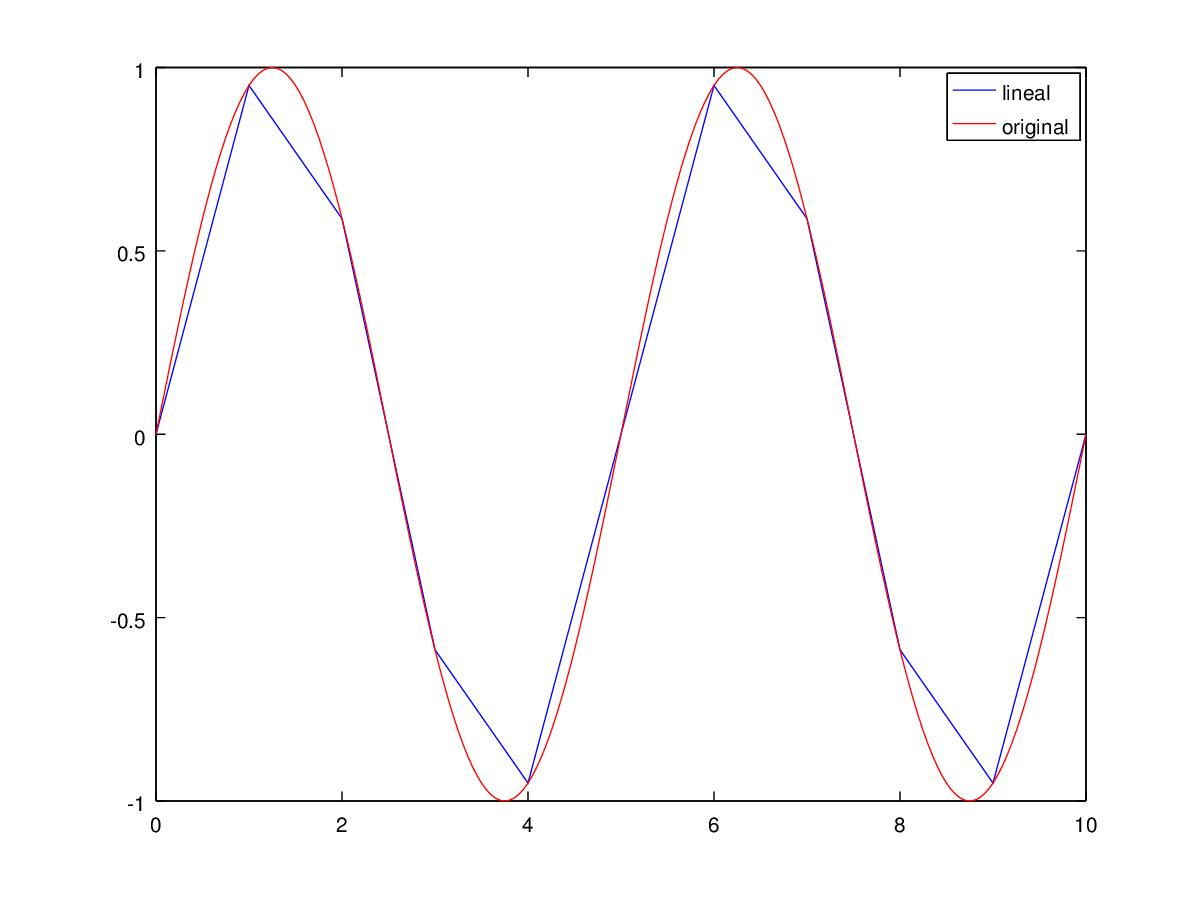
\includegraphics[width=\textwidth]{complementos/lineal_1.jpg}
    \caption{Interpolación lineal: Paso: 1.0}
  \end{minipage}
  \begin{minipage}[b]{.5\textwidth} 
    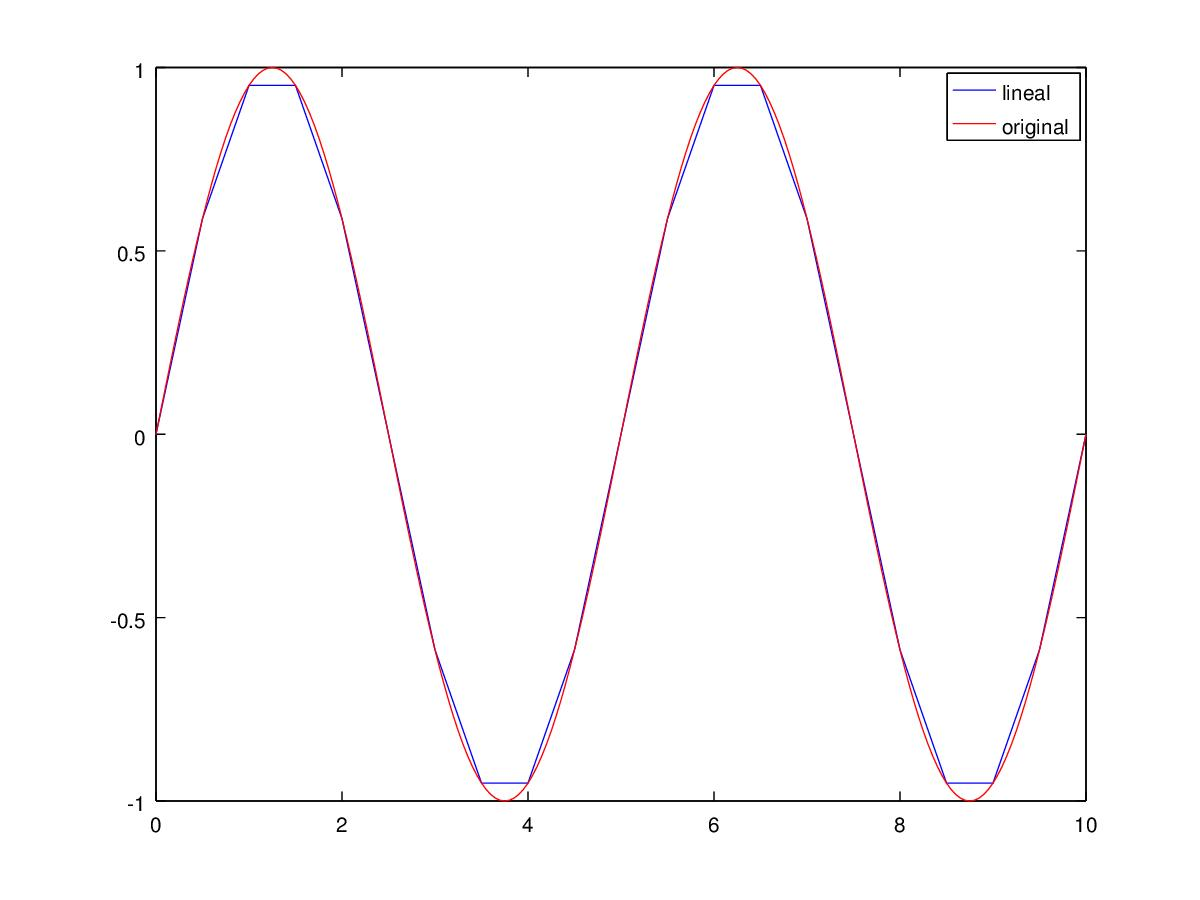
\includegraphics[width=\textwidth]{complementos/lineal_05.jpg}
    \caption{Interpolación lineal: Paso: 0.5}
  \end{minipage}
\end{figure} \label{eq:lineal_graph}

Como podemos apreciar, en la Figura 4 tomamos intervalos de la mitad del tamaño que en la Figura 3, al conocer más valores, el polinomio interpolador tiene más información de la función, lo cual hace que las rectas estén más pegadas a la función real y por lo tanto aproxime mejor para valores intermedios en cada intervalo. 

%En la interpolación linel se utiliza un segmento rectilineo que pasa por dos puntos que se conocen: $(x_0, y_0)$ y $(x_1, y_1)$. La pendiente de la recta que pasa por esos puntos será: 
\vspace{4mm}
Para cada par de puntos $(x_i, y_i)$ y $(x_{i+1}, y_{i+1})$, la recta que pasa por ellos es nada más y nada menos que la recta secante a la función en esos puntos. La pendiente de la misma se será:

\begin{equation}
	 m = \dfrac{y_{i+1} - y_i}{x_{i+1} - x_i}
\end{equation}

Luego en la ecuación de la recta $y = m(x - x_i) + y_i$ podemos sustituir $m$ y 
obtener:

\begin{equation} \label{eq:lineal}
	 y = P(x) = y_i + (y_{i+1} - y_i)\dfrac{y_{i+1} - y_i}{x_{i+1} - x_i} 
\end{equation} 

Donde (\ref{eq:lineal}) es un polinomio de grado 1 y si evaluamos en $x_i$ y $x_{i+1}$ respectivamente obtenemos:

\begin{equation}
	 P(x_0) = y_i + (y_{i+1} - y_i)(0) = y_i \wedge P(x_{i+1}) = y_i + (y_{i+1} - y_i)(1) = y_{i+1} 
\end{equation}

Luego dados $n$ puntos de la función podemos definir un polinomio como una función partida entre cada par de puntos para los cuales se obtendrá una recta que los interpole

 \begin{displaymath}
   P(x) = \left\{
     \begin{array}{lr}
       y_0 + (y_1 - y_0)\dfrac{y_1 - y_0}{x_1 - x_0}  & : x_0 \leq x < x_1\\\\
       y_1 + (y_2 - y_1)\dfrac{y_2 - y_1}{x_2 - x_1}  & : x_1 \leq x < x_2\\
       \vdots\\
       y_{n-1} + (y_n - y_{n-1})\dfrac{y_n - y_{n-1}}{x_n - x_{n-1}}  & : x_{n-1}	 \leq x_i \leq x_n\\
     \end{array}
   \right.
\end{displaymath} 

Un deatalle importante es que el polinomio definido de esta manera es continuo pero no es deribable en los extremos de los intervalos. Esto se traduce directamente en que la aproximación no es "suave". Esto se puede ver con facilidad en las Figuras 3 y 4 (\ref{eq:lineal_graph}).

\subsubsection{Spline Cúbico}

Este método al igual que el anterior se basa en particionar nuestro intervalo de interes en subintervalos más pequeños con la intención de construir un polinimio particular para cada uno de estos. Se busca entonces que para cada subintevalo, su polinomio asociado aproxime a la función estudiada en el interior del mismo, y además coincida con los resultados ya conocidos en ambos extremos. 

Nuestra partición a considerar será la inducida por $a = x_0 < x_1 \dots < x_n = b$, es decir, las pre-imagenes ordenadas de menor a mayor de los valores ya conocidos de \textit{f}; y nuestros polinomios serán polinomios cúbicos que cumplan ciertas propiedades, entre las cuales, que los extremos coincidan con los polinomios de los intervalos vecinos, y además también coincidan sus primeras y segundas derivadas; como resultado obtenemos sobre todo el intervalo original una función continua y de derivadas primera y segunda también continuas, es decir de clase $C^{2}[a, b]$. No obstante, no necesariamente ocurre que estas derivadas concuerden con las de la función a interpolar, ni siquiera que las aproximen.

%La alternativa se basa en dividir el intervalo en subintervalos y construir en cada uno de ellos un polinomio. Generalmente se denomina a esta técnica interpolación por partes. La mas común y usada es la que utiliza polinomios de grado tres y se denomina spline cúbico. 
%Al ser un polinomio cúbico hay suficiente flexibilidad para asegurar que la interpolación es clase $C^{2}[a, b]$, es decir, que es continua y tiene primeras y segundas derivadas, aunque no por esto asume que vayan a coincidir con los de la función aproximada.

Expresando lo anterior de manera formal, tenemos que, dada una función $f$ definida en $[a, b]$ y los puntos $a = x_0 < x_1 \dots < x_n = b$ un spline cúbico $S$ para $f$ es un polinomio que satisface las siguientes condiciones:

\begin{enumerate}
\item $S(x)$ es un polinomio cúbico, denotado $S_j(x)$ en el intervalo $[x_j, x_{j+1}] \forall j = 0, 1, \dots, n-1$ \label{eq:s1}
\item $S_j(x) = f(x_j)$ y $S_j(x_{j+1}) = f(x_{j+1})$ $\forall j = 0, 1, \dots, n-1$ con $S_j(x) = a_j + b_j(x - x_j) + c_j(x - x_j)^2 + d_j(x - x_j)^3$ \label{eq:s2}
\item $S_{j+1}(x_{j+1}) = S_j(x_{j+1})$ $\forall j = 0, 1, \dots, n-2$ \label{eq:s3}
\item $S_{j+1}^{'}(x_{j+1}) = S_j^{'}(x_{j+1})$ $\forall j = 0, 1, \dots, n-2$ \label{eq:s4}
\item $S_{j+1}^{''}(x_{j+1}) = S_j^{''}(x_{j+1})$ $\forall j = 0, 1, \dots, n-2$ \label{eq:s5}
\item Una de las siguientes condiciones necesita ser cumplida \label{eq:s6}
\subitem 1) $S^{''}(x_0) = S^{''}(x_n) = 0$ (borde natural) 
\subitem 2) $S^{'}(x_0) =  f^{'}(x_0) \wedge S^{'}(x_n) = f^{'}(x_n)$ (borde sujeto) 
\end{enumerate}

Observemos que se necesita cumplir con una de las dos condiciones de (\ref{eq:s6}), ahora bien, en particular satisfacer 2) dará como resultado una aproximación más precisa de la función real, dado que estamos utilizando más información de la misma, pero para ello necesitaremos conocer los valores de la derivada de la función en esos puntos y esto en general no suele suceder. Este será el caso de este trabajo práctico, por lo cual utilizaremos 1), dado que solo debemos garantizar una propiedad sobre datos conocidos.

Veamos como se comporta la función $sen(2\pi(x/5))$ con spline natural

\pagebreak

\begin{figure}[h]
\centering
  \begin{minipage}[b]{.9\textwidth}
    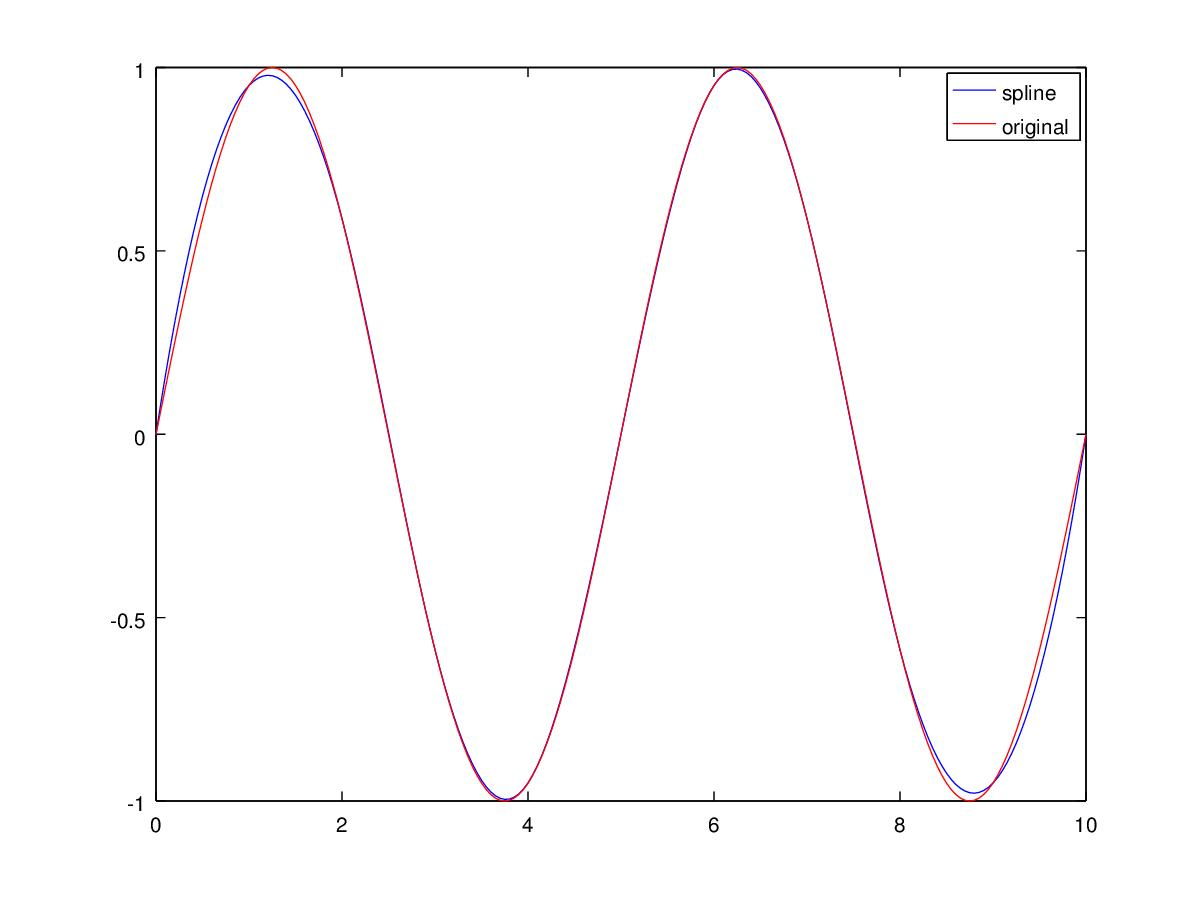
\includegraphics[width=\textwidth]{complementos/spline_1.jpg}
    \caption{Interpolación splines cúbicos: Paso: 1.0}
  \end{minipage}
\end{figure}

Parece bastante claro que se ajusta mucho mejor a la función original que interpolación lineal. Esto se debe a las condiciones pedidas sobre los extremos de los intervalos, logrando que las curvas sean suaves en comparación a los picos obtenidos con lineal. 

En general, trabajar con splines siempre será lo ideal debido que no siempre contaremos con la cantidad suficiente de información sobre la función que estamos interpolando como para lograr que lineal aproxime correctamente. 

\section{Slow Motion: Modelado}

\subsection{El objetivo inicial}

Como mencionamos en la introducción el objetivo de este trabajo práctico es generar videos en cámara lenta basandonos en la idea de introducir cuadros intermedios generados con los métodos mencionados de interpolación. Veremos ahora como representar un video para poder lograrlo y luego aplicaremos cada método y observaremos que sucede en cada caso.

\subsection{Manipilación de los cuadros: interpolando imágenes}

Un video está compuesto por cuadros, que no son más que las imágenes de las que se compone el video   y que serán determinadas por la cantidad de cuadros por segundo o fps a la que el video se reproduce y la duración del mismo.
Por ejemplo si el video se reproduce a 30 fps y dura 5 segundos, tendremos 150 cuadros en total y dado que 1 sg = 1000 ms, cada imágen se verá en pantalla por aproximadamente 33,33 ms.

Cada imágen está compuesta por pixeles que se pueden representar en matrices donde cada posicion $i$, $j$ de un cuadro $k$ representa un color en la escala de grises $[0..255]$ $\in$ $\mathbb{N}$. Los videos que utilizaremos en la experimentación serán en escala de grises por el único motivo de que disminuirá los tiempos de cómputo involucrados en comparación a si trabajaramos con toda la representación de colores rgb. Aunque esta misma idea puede generalizarse y adaptarse para todos los colores sin inconveniente alguno.
La matriz que describe un cuadro puede escribirse de la siguiente manera

\vspace{4mm}

$
\hspace{1.3cm}
     \begin{pmatrix}
      f(1, 1, k) & f(1, 2, k) & \dots & f(1, n, k) \\
	  f(2, 1, k) & f(2, 2, k) & \dots & f(2, n, k) \\
	  \vdots & \vdots & \ddots & \vdots \\
	  f(m, 1, k) & f(m, 2, k) & \dots & f(m, n, k) \\
     \end{pmatrix}
$

\vspace{4mm}

Donde $f(i, j, k)$ $\in$ $[0..255]$

Lo que haremos una vez obtenidos los cuadros que representan el video será interpolar entre cada par de posiciones para un mismo cuadro. Es decir para cada $f(i, j, k)$, $f(i, j, k+1)$ $\forall$ $k = 0, 1, \dots, n-1$ generaremos un polinomio interpolador para poder aproximar los valores intermedios a los cuadros $k$ y $k+1$.

\subsection{Discretización}

El tamaño del paso del polinomio estará determinado por la cantidad de cuadros que queramos generar entre cada par de cuadros, es decir que podriamos generar más de un cuadro intermedio, ergo, el paso será más pequeño. Como condición general el paso será el mismo para todos los polinomios. 

Dependiendo del método elegido, tomar más cuadros puede resultar beneficioso para la fluidez del resultado, pero esto en principio no será siempre así. Veremos que para los polinomios lineales esto no producirá ningún tipo de mejora y en cambio serán mejores los resultados obtenidos en interpolación cuadrática y spline cúbico. Además en general, cuanto más pequeño sea el paso involucrado, más costoso será obtener el resultado de la interpolación. Existirá como no podia ser de otra manera un trade-off entre complejidad, eficiencia, suavidad y nitidez del resultado final. 

\subsection{Nearest Neighbour}

Introduciremos aquí un método que aunque podría considerarse poco efectivo, nos servirá para tener un margen más amplio de comparación. El mismo se basa en la idea de que tambien podemos interpolar copiando el cuadro más cercano entre dos cuadros $k$ y $k+1$. Este método se denomina Nearest Neighbour. 

Además no solo está limitado a la generación de un cuadro intermedio. Aquí tambien podremos utilizar el paso como parámetro. Dado que este método no utiliza un polinomio para aproximar valores, lo que haremos será partir a la mitad el intervalo (más, menos uno, esto será determinado en la experimentación) y replicar el cuadro izquierdo tantas veces como paso/2 y lo mismo con el cuadro derecho. 

\subsection{El modelo empírico}

Para poder valorar el resultado de las experimentaciones correctamente no basta con un análisis subjetivo de comparación de los métodos entre si. Necesitamos poder comparar con un módelo empírico que nos de una idea más objetiva de como se comporta cada interpolación. Para esto mismo consideraremos un video del que obtendremos sus cuadros tomando saltos equidistantes, por ejemplo, eliminado los cuadros impares, sin eliminar el primero y el último ya que los bordes siempre estarán incluidos. Luego interpolaremos los cuadros faltantes con cada uno de los métodos y tomaremos las siguientes medidas:

\begin{equation}
	PSNR = 10 \times log_{10}(\dfrac{MAX_u^2}{ECM})
\end{equation}

Donde $MAX_u$ define el rango máximo de la imágen, es decir, 255 y $ECM$ el error cuadrático medio

\begin{equation}
	\dfrac{1}{N}\sum_{i,j}(u_{ij}^* - u_{ij})^2
\end{equation}

Donde $N$ es la cantidad de pixeles de la imágen, $u^*$ es la imágen ideal y $u$ es la imágen que construimos. Este error es bastante intuitivo y tiene mucha aplicación en estadistica. Nos da una idea del error cometido al aproximar todos los valores de la imágen ideal. 

El $PSNR$ es algo menos intuitivo. Sus siglas provienen de Peak Signal-to-Noise Ratio que en español significa Relación Señal a Ruido de Pico. Suele usarse en el ámbito de la compresión de imágenes y es la medida cuantitativa de la calidad de la reconstrucción. Lo que define es la relación entre la máxima energía posible de una señal y el ruido que afecta a su representación fidedigna. 
Tiene aplicación en esta experimentación dado que lo que haremos tambien será reconstruir parte del video.

De esta manera podremos saber que método aproxima mejor al resultado ideal de manera objetiva. 

(redondear un poco más todo esto...le falta)










